\chapter{Variational-Net Solutions}
\begin{enumerate}
	\item A double pendulum consists of two point masses $m$ attached by strings of length $l$ as shown in the figure: The kinetic energy of the pendulum is
	{\exyear{NET/JRF(DEC-2011)}}
\begin{figure}[H]
\centering
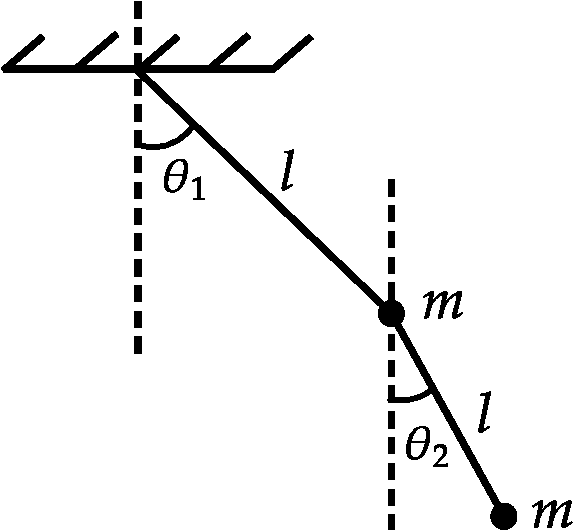
\includegraphics[height=4cm,width=4.5cm]{diagram-20210926(1)-crop}
\end{figure}
\begin{tasks}(1)
\task[\textbf{A.}] $\frac{1}{2} m l^{2}\left[\dot{\theta}_{1}^{2}+\dot{\theta}_{2}^{2}\right]$
\task[\textbf{B.}] $\frac{1}{2} m l^{2}\left[2 \dot{\theta}_{1}^{2}+\dot{\theta}_{2}^{2}+2 \dot{\theta}_{1} \dot{\theta}_{2} \cos \left(\theta_{1}-\theta_{2}\right)\right]$
\task[\textbf{C.}] $\frac{1}{2} m l^{2}\left[\dot{\theta}_{1}^{2}+2 \dot{\theta}_{2}^{2}+2 \dot{\theta}_{1} \dot{\theta}_{2} \cos \left(\theta_{1}-\theta_{2}\right)\right]$
\task[\textbf{D.}] $\frac{1}{2} m l^{2}\left[2 \dot{\theta}_{1}^{2}+\dot{\theta}_{2}^{2}+2 \dot{\theta}_{1} \dot{\theta}_{2} \cos \left(\theta_{1}+\theta_{2}\right)\right]$
\end{tasks}
\begin{answer}
\begin{align*}
\text{	Let co-ordinate }&\left(x_{1}, y_{1}\right)\text{ and }\left(x_{2}, y_{2}\right) .\\ K . E .&=\frac{1}{2} m\left(\dot{x}_{1}^{2}+\dot{y}_{1}^{2}\right)+\frac{1}{2} m\left(\dot{x}_{2}^{2}+\dot{y}_{2}^{2}\right)\\
x_{1}&=l \sin \theta_{1}, y_{1}=l \cos \theta_{1} \Rightarrow \dot{x}_{1}\\&=l \cos \theta_{1} \dot{\theta}_{1}, \dot{y}_{1}=-l \sin \theta_{1} \dot{\theta}_{1}\\
x_{2}&=l \sin \theta_{1}+l \sin \theta_{2}, y_{2}=l \cos \theta_{1}+l \cos \theta_{2}\\
\Rightarrow \dot{x}_{2}&=l \cos \theta_{1} \dot{\theta}_{1}+l \cos \theta_{2} \dot{\theta}_{2}, \dot{y}_{2}\\&=l\left(-\sin \theta_{1} \dot{\theta}_{1}\right)+l\left(-\sin \theta_{2}\right) \dot{\theta}_{2}
\intertext{Put the value of $\dot{x}_{1}, \dot{y}_{1}, \dot{x}_{2}, \dot{y}_{2}$ in K.E equation, one will get}
T&=\frac{1}{2} m l^{2}\left[2 \dot{\theta}_{1}^{2}+\dot{\theta}_{2}^{2}+2 \dot{\theta}_{1} \dot{\theta}_{2} \cos \left(\theta_{1}-\theta_{2}\right)\right]
\end{align*}
So the correct answer is \textbf{Option (B)}
\end{answer}
\item A particle of mass $m$ moves inside a bowl. If the surface of the bowl is given by the equation $z=\frac{1}{2} a\left(x^{2}+y^{2}\right)$, where $a$ is a constant, the Lagrangian of the particle is
{\exyear{NET/JRF(DEC-2011)}}
\begin{tasks}(2)
\task[\textbf{A.}] $\frac{1}{2} m\left(\dot{r}^{2}+r^{2} \dot{\phi}^{2}-g a r^{2}\right)$
\task[\textbf{B.}] $\frac{1}{2} m\left[\left(1+a^{2} r^{2}\right) \dot{r}^{2}+r^{2} \dot{\phi}^{2}\right]$
\task[\textbf{C.}]  $\frac{1}{2} m\left(\dot{r}^{2}+r^{2} \dot{\theta}^{2}+r^{2} \sin ^{2} \theta \dot{\phi}^{2}-g a r^{2}\right)$
\task[\textbf{D.}]  $\frac{1}{2} m\left[\left(1+a^{2} r^{2}\right) \dot{r}^{2}+r^{2} \dot{\phi}^{2}-g a r^{2}\right]$
\end{tasks}
\begin{answer}
\begin{align*}
L&=\frac{1}{2} m\left(\dot{x}^{2}+\dot{y}^{2}+\dot{z}^{2}\right)-m g z,\\\text{ where } z&=\frac{1}{2} a\left(x^{2}+y^{2}\right)\\
\text{It has cylindrical symmetry. Thus }x&=r \cos \phi, y=r \sin \phi, z=\frac{1}{2} a\left(r^{2}\right)\\
\dot{x}&=\dot{r} \cos \phi-r \sin \phi \dot{\phi}, \dot{y}\\&=\dot{r} \sin \phi+r \cos \phi \dot{\phi}\text{ and }\dot{z}=a(r \dot{r})\\
\text{	So, }L&=\frac{1}{2} m\left[\left(1+a^{2} r^{2}\right) \dot{r}^{2}+r^{2} \dot{\phi}^{2}-g a r^{2}\right]
\end{align*}
So the correct answer is \textbf{Option (D)}
\end{answer}
\item The Lagrangian of a particle of mass $m$ moving in one dimension is given by
$$
L=\frac{1}{2} m \dot{x}^{2}-b x
$$
where $b$ is a positive constant. The coordinate of the particle $x(t)$ at time $t$ is given by: (in following $c_{1}$ and $c_{2}$ are constants)
{\exyear{NET/JRF(JUNE-2013)}}
\begin{tasks}(2)
\task[\textbf{A.}] $-\frac{b}{2 m} t^{2}+c_{1} t+c_{2}$
\task[\textbf{B.}] $c_{1} t+c_{2}$
\task[\textbf{C.}] $c_{1} \cos \left(\frac{b t}{m}\right)+c_{2} \sin \left(\frac{b t}{m}\right)$
\task[\textbf{D.}] $c_{1} \cosh \left(\frac{b t}{m}\right)+c_{2} \sinh \left(\frac{b t}{m}\right)$
\end{tasks}
\begin{answer}
\begin{align*}
\text{Equation of motion }\frac{d}{d t}\left(\frac{\partial L}{\partial \dot{x}}\right)-\frac{\partial L}{\partial x}&=0 \Rightarrow \frac{d}{d t}(m \dot{x})+b\\&=0 \Rightarrow m \ddot{x}+b=0 \Rightarrow m \ddot{x}=-b\\
\frac{d^{2} x}{d t^{2}}&=-\frac{b}{m} \Rightarrow \frac{d x}{d t}=-\frac{b}{m} t+c_{1} \Rightarrow x\\&=-\frac{b}{m} \frac{t^{2}}{2}+c_{1} t+c_{2}
\end{align*}
So the correct answer is \textbf{Option (A)}
\end{answer}	
\item A particle moves in a potential $V=x^{2}+y^{2}+\frac{z^{2}}{2} .$ Which component(s) of the angular momentum is/are constant(s) of motion?
{\exyear{NET/JRF(DEC-2013)}}
\begin{tasks}(4)
\task[\textbf{A.}] None
\task[\textbf{B.}] $L_{x}, L_{y}$ and $L_{z}$
\task[\textbf{C.}]  only $L_{x}$ and $L_{y}$
\task[\textbf{D.}] only $L_{z}$
\end{tasks}
\begin{answer}
\begin{align*}
\text{A particle moves in a potential }V&=x^{2}+y^{2}+\frac{z^{2}}{2}\\
V(r, \theta, \phi)&=r^{2} \sin ^{2} \theta \cos ^{2} \phi+r^{2} \sin ^{2} \theta \sin ^{2} \phi+\frac{r^{2}}{2} \cos ^{2} \theta\\
V(r, \theta, \phi)&=r^{2} \sin ^{2} \theta+\frac{r^{2}}{2} \cos ^{2} \theta\\
\text{	Now $\phi$ is cyclic-co-ordinate }&\left(p_{\phi}\right)\text{ i.e $L_{z}$ is constant of motion.}
\end{align*}
So the correct answer is \textbf{Option (D)}
\end{answer}
\item A pendulum consists of a ring of mass $M$ and radius $R$ suspended by a massless rigid rod of length $l$ attached to its rim. When the pendulum oscillates in the plane of the ring, the time period of oscillation is
{\exyear{NET/JRF(DEC-2013)}}
\begin{tasks}(2)
\task[\textbf{A.}] $2 \pi \sqrt{\frac{l+R}{g}}$
\task[\textbf{B.}] $\frac{2 \pi}{\sqrt{g}}\left(l^{2}+R^{2}\right)^{1 / 4}$
\task[\textbf{C.}] $2 \pi \sqrt{\frac{2 R^{2}+2 R l+l^{2}}{g(R+l)}}$
\task[\textbf{D.}] $\frac{2 \pi}{\sqrt{g}}\left(2 R^{2}+2 R l+l^{2}\right)^{1 / 4}$
\end{tasks}
\begin{answer}
\begin{align*}
\intertext{The moment of inertia about pivotal point is given by}
I&=I_{c, m}+M d^{2}=M R^{2}+M(l+R)^{2}\\
\intertext{If ring is displaced by angle $\theta$ then potential energy is $-M g(l+R) \cos \theta$.}
\intertext{ The Lagrangian is given by}
L&=\frac{1}{2} I \dot{\theta}^{2}-V(\theta)\\&=\frac{1}{2}\left(M R^{2}+M(l+R)^{2}\right) \dot{\theta}^{2}+M g(l+R) \cos \theta\\
\frac{d}{d t}\left(\frac{\partial L}{\partial \dot{\theta}}\right)-\left(\frac{\partial L}{\partial \theta}\right)&=0 \Rightarrow\left(M R^{2}+M(l+R)^{2}\right) \ddot{\theta}+M g(l+R) \sin \theta=0\\
\text{For small oscillation }\sin \theta&=\theta \Rightarrow\left(M R^{2}+M(l+R)^{2}\right) \ddot{\theta}+M g(l+R) \theta=0\\
\text{Time period is given by }&2 \pi \sqrt{\frac{2 R^{2}+2 R l+l^{2}}{g(R+l)}}.
\end{align*}
So the correct answer is \textbf{Option (C)}
\end{answer}	
\item Consider a particle of mass $m$ attached to two identical springs each of length $l$ and spring constant $k$ (see the figure). The equilibrium configuration is the one where the springs are unstretched. There are no other external forces on the system. If the particle is given a small displacement along the $x$-axis, which of the following describes the equation of motion for small oscillations?
{\exyear{NET/JRF(DEC-2013)}}
\begin{figure}[H]
\centering
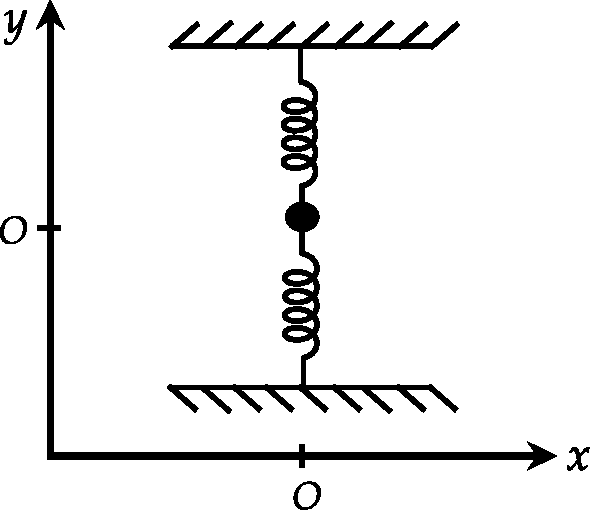
\includegraphics[height=4.5cm,width=5cm]{diagram-20210926(18)-crop}
\end{figure}
\begin{tasks}(4)
\task[\textbf{A.}] $m \ddot{x}+\frac{k x^{3}}{l^{2}}=0$
\task[\textbf{B.}]  $m \ddot{x}+k x=0$
\task[\textbf{C.}] $m \ddot{x}+2 k x=0$
\task[\textbf{D.}] $m \ddot{x}+\frac{k x^{2}}{l}=0$
\end{tasks}
\begin{answer}$\left. \right. $
\begin{figure}[H]
	\centering
	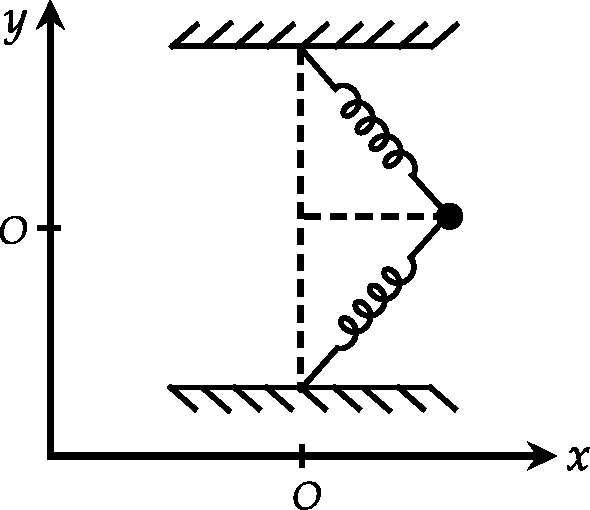
\includegraphics[height=4.5cm,width=5cm]{diagram-20210926(19)-crop}
\end{figure}
\begin{align*}
\intertext{The lagrangian of system is given by}
L&=\frac{1}{2} m \dot{x}^{2}-V(x)
\intertext{The potential energy is given by}
V(x)&=\frac{k}{2}\left[\left(x^{2}+l^{2}\right)^{\frac{1}{2}}-l\right]^{2}+\frac{k}{2}\left[\left(x^{2}+l^{2}\right)^{\frac{1}{2}}-l\right]^{2}\\
V(x)&=k\left[\left(x^{2}+l^{2}\right)^{\frac{1}{2}}-l\right]^{2}
\intertext{For small oscillation one can approximate potential by Taylor expansion}
V(x)&=k l^{2}\left[\left(1+\frac{x^{2}}{l^{2}}\right)^{\frac{1}{2}}-1\right]^{2} \Rightarrow V(x)\\&=k l^{2}\left[\left(1+\frac{1}{2} \frac{x^{2}}{l^{2}}-\frac{1}{8} \frac{x^{4}}{l^{4}}\right)-1\right]^{2}\\
V(x)&=\frac{k l^{2}}{4}\left(\frac{x^{2}}{l^{2}}\right)^{2} \Rightarrow V(x)=k\left(\frac{x^{4}}{4 l^{2}}\right)\\
\text{So Lagrangian of system is given by }L&=\frac{1}{2} m \dot{x}^{2}-k\left(\frac{x^{4}}{4 l^{2}}\right)\\
\text{The Lagranges equation of motion }&\frac{d}{d t}\left(\frac{\partial L}{\partial \dot{x}}\right)-\left(\frac{\partial L}{\partial x}\right)=0 \Rightarrow m \ddot{x}+\frac{k x^{3}}{l^{2}}=0
\end{align*}
So the correct answer is \textbf{Option (A)}
\end{answer}	
\item The equation of motion of a system described by the time-dependent Lagrangian
$$
L=e^{\gamma t}\left[\frac{1}{2} m \dot{x}^{2}-V(x)\right] \text { is }
$$
{\exyear{NET/JRF(DEC-2014)}}
\begin{tasks}(2)
\task[\textbf{A.}] $m \ddot{x}+\gamma m \dot{x}+\frac{d V}{d x}=0$
\task[\textbf{B.}] $m \ddot{x}+\gamma m \dot{x}-\frac{d V}{d x}=0$
\task[\textbf{C.}]  $m \ddot{x}-\gamma m \dot{x}+\frac{d V}{d x}=0$
\task[\textbf{D.}] $m \ddot{x}+\frac{d V}{d x}=0$
\end{tasks}
\begin{answer}
\begin{align*}
\because L&=e^{\gamma t}\left[\frac{1}{2} m \dot{x}^{2}-V(x)\right] \Rightarrow \frac{\partial L}{\partial \dot{x}}\\&=e^{\gamma t} m \dot{x}\text{ and }\frac{\partial L}{\partial x}=-\frac{\partial V}{\partial x} e^{\gamma t}\\
\because \frac{d}{d t}\left(\frac{\partial L}{\partial \dot{x}}\right)-\frac{\partial L}{\partial x}&=0 \Rightarrow \frac{d}{d t}\left(e^{\gamma t} m \dot{x}\right)+\frac{\partial V}{\partial x} e^{\gamma t}\\&=m \ddot{x} e^{r t}+m \dot{x} \gamma e^{\gamma t}+\frac{\partial V}{\partial x} e^{r t}=0\\
\left(m \ddot{x}+m \gamma \dot{x}+\frac{\partial V}{\partial x}\right) e^{\gamma t}&=0 \Rightarrow m \ddot{x}+\gamma m \dot{x}+\frac{\partial V}{\partial x}=0
\end{align*}
So the correct answer is \textbf{Option (A)}
\end{answer}	
\item A particle of unit mass moves in the $x y$-plane in such a way that $\dot{x}(t)=y(t)$ and $\dot{y}(t)=-x(t) .$ We can conclude that it is in a conservative force-field which can be derived from the potential
{\exyear{NET/JRF(JUNE-2015)}}
\begin{tasks}(4)
\task[\textbf{A.}] $\frac{1}{2}\left(x^{2}+y^{2}\right)$
\task[\textbf{B.}] $\frac{1}{2}\left(x^{2}-y^{2}\right)$
\task[\textbf{C.}] $x+y$
\task[\textbf{D.}] $x-y$
\end{tasks}
\begin{answer}
\begin{align*}
\because \dot{x}&=y\text{ and }\dot{y}=-x\\
\Rightarrow \quad \ddot{x}&=\dot{y}=-x \quad\text{ and }\ddot{y}=-\dot{x}=-y\\
\Rightarrow \quad \ddot{x}+x&=0 \quad\text{ and }\ddot{y}+y=0\\
\text{that is possible for }L&=\frac{1}{2} m \dot{x}^{2}+\frac{1}{2} m \dot{y}^{2}-\frac{1}{2}\left(x^{2}+y^{2}\right) \\\Rightarrow V&=\frac{1}{2}\left(x^{2}+y^{2}\right)
\end{align*}
So the correct answer is \textbf{Option (A)}
\end{answer}	
\item The Lagrangian of a particle moving in a plane s given in Cartesian coordinates as
$$
L=\dot{x} \dot{y}-x^{2}-y^{2}
$$
In polar coordinates the expression for the canonical momentum $p_{r}$ (conjugate to the radial coordinate $r$ ) is
{\exyear{NET/JRF(DEC-2015)}}
\begin{tasks}(2)
\task[\textbf{A.}] $\dot{r} \sin \theta+r \dot{\theta} \cos \theta$
\task[\textbf{B.}]  $\dot{r} \cos \theta+r \dot{\theta} \sin \theta$
\task[\textbf{C.}] $2 \dot{r} \cos \theta-r \dot{\theta} \sin 2 \theta$
\task[\textbf{D.}] $\dot{r} \sin 2 \theta+r \dot{\theta} \cos 2 \theta$
\end{tasks}
\begin{answer}
\begin{align*}
L&=\dot{x} \dot{y}-x^{2}-y^{2}=\dot{x} \dot{y}-\left(x^{2}+y^{2}\right)\\
x&=r \cos \theta, y=r \sin \theta \Rightarrow \dot{x}=\dot{r} \cos \theta-r \sin \theta \dot{\theta}, \\ \dot{y}&=\dot{r} \sin \theta+r \cos \theta \dot{\theta}\\
L&=\dot{r}^{2} \sin \theta \cos \theta-r^{2} \sin \theta \cos \theta \dot{\theta}^{2}+\dot{r} r \cos ^{2} \theta \dot{\theta}-\dot{r} r \sin ^{2} \theta \dot{\theta}\\
P_{r}&=\frac{\partial L}{\partial \dot{r}} \Rightarrow 2 \dot{r} \sin \theta \cos \theta+r \dot{\theta}\left(\cos ^{2} \theta-\sin ^{2} \theta\right)\\
\Rightarrow P_{r}&=\dot{r} \sin 2 \theta+r \dot{\theta} \cos 2 \theta
\end{align*}
So the correct answer is \textbf{Option (D)}
\end{answer}
\item The dynamics of a particle governed by the Lagrangian
$$
L=\frac{1}{2} m \dot{x}^{2}-\frac{1}{2} k x^{2}-k x \dot{x} t \text { describes }
$$
{\exyear{NET/JRF(DEC-2016)}}
\begin{tasks}(1)
\task[\textbf{A.}] An undamped simple harmonic oscillator
\task[\textbf{B.}] A damped harmonic oscillator with a time varying damping factor
\task[\textbf{C.}]  An undamped harmonic oscillator with a time dependent frequency
\task[\textbf{D.}] A free particle
\end{tasks}
\begin{answer}
\begin{align*}
L&=\frac{1}{2} m \dot{x}^{2}-\frac{1}{2} k x^{2}-k x \dot{x} t\\
\frac{\partial L}{\partial \dot{x}}&=m \dot{x}-k x t, \frac{\partial L}{\partial x}=-k x-k \dot{x} t\\
\frac{d}{d t}\left(\frac{\partial L}{\partial \dot{x}}\right)-\frac{\partial L}{\partial x}&=0 \Rightarrow m \ddot{x}-k \dot{x} t-k x+k x+k \dot{x} t\\&=0 \Rightarrow m \ddot{x}=0
\intertext{So motion is equivalent to free particle}
\end{align*}
So the correct answer is \textbf{Option (D)}
\end{answer}	
\item The parabolic coordinates $(\xi, \eta)$ are related to the Cartesian coordinates $(x, y)$ by $x=\xi \eta$ and $y=\frac{1}{2}\left(\xi^{2}-\eta^{2}\right)$. The Lagrangian of a two-dimensional simple harmonic oscillator of mass $m$ and angular frequency $\omega$ is
{\exyear{NET/JRF(DEC-2016)}}
\begin{tasks}(2)
\task[\textbf{A.}] $\frac{1}{2} m\left[\dot{\xi}^{2}+\dot{\eta}^{2}-\omega^{2}\left(\xi^{2}+\eta^{2}\right)\right]$
\task[\textbf{B.}] $\frac{1}{2} m\left(\xi^{2}+\eta^{2}\right)\left[\left(\dot{\xi}^{2}+\dot{\eta}^{2}\right)-\frac{1}{4} \omega^{2}\left(\xi^{2}+\eta^{2}\right)\right]$
\task[\textbf{C.}] $\frac{1}{2} m\left(\xi^{2}+\eta^{2}\right)\left[\dot{\xi}^{2}+\dot{\eta}^{2}-\frac{1}{2} \omega^{2} \xi \eta\right]$
\task[\textbf{D.}] $\frac{1}{2} m\left(\xi^{2}+\eta^{2}\right)\left[\dot{\xi}^{2}+\dot{\eta}^{2}-\frac{1}{4} \omega^{2}\right]$
\end{tasks}
\begin{answer}
\begin{align*}
\intertext{For two dimensional Harmonic oscillation}
L&=\frac{1}{2} m\left(\dot{x}^{2}+\dot{y}^{2}\right)-\frac{1}{2} m \omega^{2}\left(x^{2}+y^{2}\right)\\
x&=\xi \eta, \quad y=\frac{1}{2}\left(\xi^{2}-\eta^{2}\right)\\
\dot{x}&=\dot{\xi} \eta+\xi \dot{\eta}, \quad \dot{y}=\xi \dot{\xi}-\eta \dot{\eta}\\
L&=\frac{1}{2} m\left[(\dot{\xi} \eta+\xi \dot{\eta})^{2}+(\xi \dot{\xi}-\eta \dot{\eta})^{2}\right]-\frac{1}{2} m \omega^{2}\left[\xi^{2} \eta^{2}+\frac{1}{4}\left(\xi^{2}-\eta^{2}\right)^{2}\right]\\
L&=\frac{1}{2} m\left(\dot{\xi}^{2} \eta^{2}+\xi^{2} \dot{\eta}^{2}+\xi^{2} \dot{\xi}^{2}+\eta^{2} \dot{\eta}^{2}\right)-\frac{1}{8} m \omega^{2}\left(\xi^{4}+\eta^{4}+2 \xi^{2} \eta^{2}\right)\\
&=\frac{1}{2} m\left(\xi^{2}+\eta^{2}\right)\left(\dot{\eta}^{2}+\dot{\xi}^{2}\right)-\frac{1}{8} m \omega^{2}\left(\xi^{2}+\eta^{2}\right)^{2}\\
&=\frac{1}{2} m\left(\xi^{2}+\eta^{2}\right)\left[\dot{\eta}^{2}+\dot{\xi}^{2}-\frac{1}{4} \omega^{2}\left(\xi^{2}+\eta^{2}\right)\right]
\end{align*}
So the correct answer is \textbf{Option (B)}
\end{answer}	
\item The spring constant $k$ of a spring of mass $m_{s}$ is determined experimentally by loading the spring with mass $M$ and recording the time period $T$, for a single oscillation. If the experiment is carried out for different masses, then the graph that correctly represents the result is
{\exyear{NET/JRF(DEC-2017)}}
\begin{tasks}(2)
\task[\textbf{A.}] \begin{figure}[H]
	\centering
	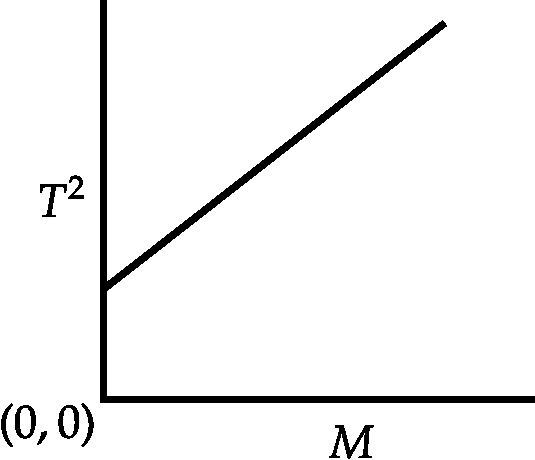
\includegraphics[height=3cm,width=4.5cm]{diagram-20210926(38)-crop}
\end{figure}
\task[\textbf{B.}] \begin{figure}[H]
	\centering
	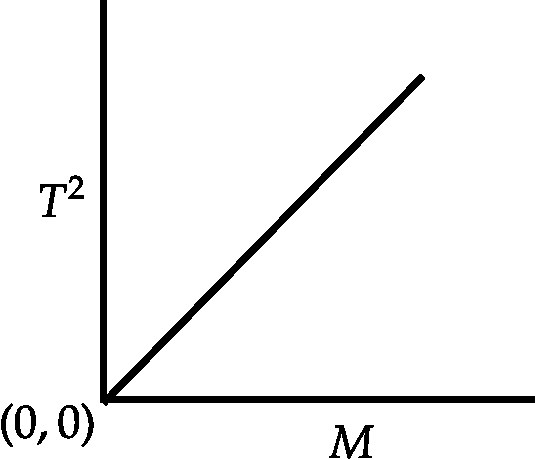
\includegraphics[height=3cm,width=4.5cm]{diagram-20210926(39)-crop}
\end{figure}
\task[\textbf{C.}] \begin{figure}[H]
	\centering
	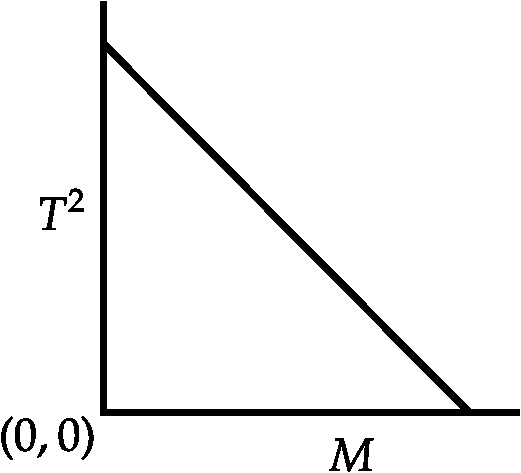
\includegraphics[height=3cm,width=4.5cm]{diagram-20210926(40)-crop}
\end{figure}
\task[\textbf{D.}] \begin{figure}[H]
	\centering
	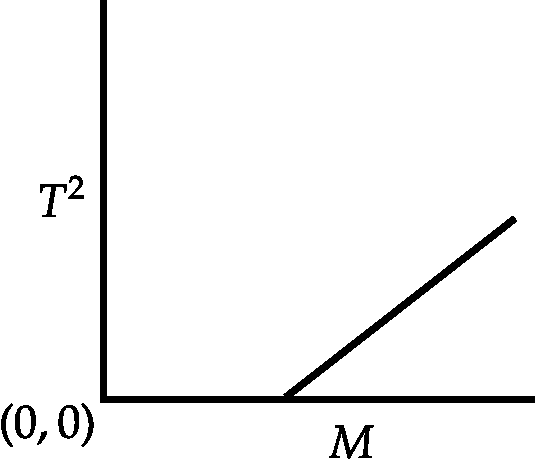
\includegraphics[height=3cm,width=4.5cm]{diagram-20210926(41)-crop}
\end{figure}
\end{tasks}
\begin{answer}
\begin{align*}
\intertext{The Langragian of system.}
L&=\frac{1}{2} \cdot \frac{m_{s}}{3} \dot{x}^{2}+\frac{1}{2} M \dot{x}^{2}-\frac{1}{2} k x^{2}, \frac{d}{d t}\left(\frac{\partial L}{\partial \dot{x}}\right)-\frac{\partial L}{\partial x}=0\\
\frac{d}{d t} \frac{\partial L}{\partial x}&=0 \Rightarrow\left(\frac{m_{s}}{3}+M\right) \ddot{x}=-k x\\
T&=2 \pi \sqrt{\frac{M+\frac{m_{s}}{3}}{k}} \Rightarrow T^{2}=4 \pi \frac{\left(M+\frac{m_{s}}{3}\right)}{k}
\end{align*}
So the correct answer is \textbf{Option (A)}
\end{answer}	
\item The motion of a particle in one dimension is described by the Langrangian $L=\frac{1}{2}\left(\left(\frac{d x}{d t}\right)^{2}-x^{2}\right)$ in suitable units. The value of the action along the classical path from $x=0$ at $t=0$ to $x=x_{0}$ at $t=t_{0}$, is
{\exyear{NET/JRF(DEC-2018)}}
\begin{tasks}(4)
\task[\textbf{A.}] $\frac{x_{0}^{2}}{2 \sin ^{2} t_{0}}$
\task[\textbf{B.}] $\frac{1}{2} x_{0}^{2} \tan t_{0}$
\task[\textbf{C.}] $\frac{1}{2} x_{0}^{2} \cot t_{0}$
\task[\textbf{D.}] $\frac{x_{0}^{2}}{2 \cos ^{2} t_{0}}$
\end{tasks}
\begin{answer}
\begin{align*}
L&=\frac{1}{2} \dot{x}^{2}-\frac{1}{2} x^{2}\\
\intertext{From Lagrangian equation of motion, $\frac{d}{d t}\left(\frac{\partial L}{\partial \dot{x}}\right)-\frac{\partial L}{\partial x}=0$}
\ddot{x}+x&=0\\
\text{The solution is}&=A \sin t+B \cos t\\
t&=0, \quad x=0, \quad B=0\\
x&=A \sin t\\
t&=t_{0}, \quad x=x_{0}, A=\frac{x_{0}}{\sin t_{0}}\\
x&=\frac{x_{0}}{\sin t_{0}} \sin t, \quad \dot{x}=\frac{x_{0}}{\sin t_{0}} \cos t\\
A&=\int_{0}^{t_{0}} L d t=\int_{0}^{t_{0}} \frac{1}{2} \dot{x}^{2} d t-\int_{0}^{t_{0}} \frac{1}{2} x^{2} d t\\&=\frac{1}{2} \frac{x_{0}^{2}}{\sin ^{2} t_{0}} \int_{0}^{t_{0}} \cos ^{2} t d t-\frac{1}{2} \frac{x_{0}^{2}}{\sin ^{2} t_{0}} \int_{0}^{t_{0}} \sin ^{2} t d t\\
&=\frac{1}{2} \frac{x_{0}^{2}}{\sin ^{2} t_{0}}\left[\int_{0}^{t_{0}} \cos ^{2} t d t-\int_{0}^{t} \sin ^{2} t d t\right]\\&=\frac{1}{2} \frac{x_{0}^{2}}{\sin ^{2} t_{0}} \int_{t}^{t_{0}} \cos 2 t d t=\left.\frac{1}{2} \frac{x_{0}^{2}}{\sin ^{2} t_{0}} \frac{\sin 2 t_{0}}{2}\right|_{0} ^{t_{0}}=\frac{x_{0}^{2}}{2} \cot t_{0}
\end{align*}
So the correct answer is \textbf{Option (C)}
\end{answer}	
\item Two particles of masses $m_{1}$ and $m_{2}$ are connected by a massless thread of length $l$ as shown in figure below.\\
The particle of mass in on the plane undergoes a circular motion with radius $r_{0}$ and angular momentum $L$. When a small radial displacement $\in$ (whew $\in \ll<r_{0}$ ) is applied, its radial coordinate is found to oscillate about $r_{0}$. The frequency of the oscillations is
{\exyear{NET/JRF(JUNE-2019)}}
\begin{tasks}(2)
\task[\textbf{A.}] $\sqrt{\frac{7 m_{2} g}{\left(m_{1}+\frac{m_{2}}{2}\right) r_{0}}}$
\task[\textbf{B.}] $\sqrt{\frac{7 m_{2} g}{\left(m_{1}+m_{2}\right) r_{0}}}$
\task[\textbf{C.}] $\sqrt{\frac{3 m_{2} g}{\left(m_{1}+\frac{m_{2}}{2}\right) r_{0}}}$
\task[\textbf{D.}] $\sqrt{\frac{3 m_{2} g}{\left(m_{1}+m_{2}\right) r_{0}}}$
\end{tasks}
\begin{answer}
\begin{align*}
L&=\frac{1}{2}\left(m_{1}+m_{2}\right) \ddot{r}+\frac{1}{2} m_{1} r^{2} \dot{\theta}^{2}-m_{2} g(l-r)\\
\text{Lagrangian equation of motion; }&\frac{d}{d t}\left(\frac{\partial L}{\partial \dot{r}}\right)-\frac{\partial L}{\partial r}=0\\
\left(m_{1}+m_{2}\right) \ddot{r}-m_{1} r \dot{\theta}^{2}+m_{2} g&=0
\intertext{Hence angular momentum is conserved}
m_{1} r^{2} \dot{\theta}&=m_{1} r_{0}^{2} \dot{\theta}_{0} \Rightarrow \dot{\theta}=\frac{r_{0}^{2} \dot{\theta}_{0}}{r^{2}}\\
\text{For circular motion }&m r_{0} \dot{\theta}_{0}^{2}=m_{2} g\\
\text{	so }r \dot{\theta}^{2}&=\frac{m_{2}}{m_{1}}\left(\frac{r_{0}}{r}\right)^{3} g\\
\left(m_{1}+m_{2}\right) \ddot{r}-m_{2}\left(\frac{r_{0}}{r}\right)^{3} g+m_{2} g&=0\\
\text{Put }r&=r_{0}+\in \ddot{r}=\ddot{\epsilon}\\
\intertext{$\left(m_{1}+m_{2}\right) \ddot{\in}-m_{2}\left(\frac{r_{0}}{r_{0}+\epsilon}\right)^{3} g+m_{2} g\Rightarrow\left(m_{1}+m_{2}\right) \ddot{\in}-m_{2} r_{0}^{3}\left(r_{0}+\epsilon\right)^{-3} g+m_{2} g$}\\
\left(m_{1}+m_{2}\right) \ddot{\star}-m_{2} r_{0}^{3} g r_{0}^{-3}\left(1+\frac{\epsilon}{r_{0}}\right)^{-3}+m_{2} g&=0\\
\left(m_{1}+m_{2}\right) \ddot+\frac{m_{2} 3 \epsilon}{r_{0}}&=0 \Rightarrow \omega=\sqrt{\frac{3 m_{2} g}{\left(m_{1}+m_{2}\right) r_{0}}}
\end{align*}
So the correct answer is \textbf{Option (D)}
\end{answer}	
\item Which of the following terms, when added to the Lagrangian $L(x, y, \dot{x}, \dot{y})$ of a system with two degrees of freedom will not change the equations of motion?\\
(check question )
{\exyear{NET/JRF(DEC-2019)}}
\begin{tasks}(4)
\task[\textbf{A.}] $x \ddot{x}-y \ddot{y}$
\task[\textbf{B.}] $x \ddot{y}-y \ddot{x}$
\task[\textbf{C.}] $x \dot{y}-y \dot{x}$
\task[\textbf{D.}] $y \dot{x}^{2}+x \dot{y}^{2}$ 
\end{tasks}
\begin{answer}
\begin{align*}
L(x, y, \dot{x}, \dot{y})\\
\frac{d}{d t}\left(\frac{\partial L}{\partial \dot{x}}\right)-\frac{\partial L}{\partial x}&=0, \frac{d}{d t}\left(\frac{\partial L}{\partial \dot{y}}\right)-\frac{\partial L}{\partial y}=0\\
L^{\prime}&=L(x, y, \dot{x}, \dot{y})+x \ddot{y}-y \ddot{x}\\
\frac{d^{\prime}}{d t^{\prime}}\left(\frac{\partial L^{\prime}}{\partial \dot{x}}\right)-\frac{\partial L^{\prime}}{\partial x}&=\frac{d}{d t}\left(\frac{\partial L}{\partial \dot{x}}\right)-\frac{\partial L}{\partial x}+\ddot{y}\\&=0=0+\ddot{y}=0 \Rightarrow \dot{y}=c_{1}\\
\frac{d}{d t}\left(\frac{\partial L}{\partial y}\right)-\frac{\partial L^{\prime}}{\partial y}&=\frac{d}{d t}\left(\frac{\partial L}{\partial \dot{y}}\right)-\frac{\partial L}{\partial y}+\ddot{x}\\&=0=0-\ddot{x}=0 \Rightarrow \dot{x}=c_{2}
\end{align*}
So the correct answer is \textbf{Option (B)}
\end{answer}	
\item A point mass $m$, is constrained to move on the inner surface of a paraboloid of revolution $x^{2}+y^{2}=a z$ (where $a>0$ is a constant). When it spirals down the surface, under the influence of gravity (along $-z$ direction), the angular speed about the $z$-axis is proportional to
{\exyear{NET/JRF(JUNE-2020)}}
\begin{tasks}(2)
\task[\textbf{A.}] 1 (independent of $z$ )
\task[\textbf{B.}] $z$
\task[\textbf{C.}]  $z^{-1}$
\task[\textbf{D.}] $z^{-2}$
\end{tasks}
\begin{answer}
\begin{align*}
\intertext{Using Lagrangian in cylindrical coordinate}
L&=\frac{1}{2} m\left(\dot{r}^{2}+r^{2} \dot{\theta}^{2}+\dot{z}^{2}\right)-m g z \\\text{ with constraint }x^{2}+y^{2}&=a z \Rightarrow r^{2}=a z \Rightarrow \dot{z}=\frac{2 r \dot{r}}{a}\\
L&=\frac{1}{2} m\left(\dot{r}^{2}+r^{2} \dot{\theta}^{2}+\left(\frac{2 r \dot{r}}{a}\right)^{2}\right)-\frac{m g r^{2}}{a}\\
\theta \text{is cyclic coordinate so }\frac{\partial L}{\partial \theta}&=0 \Rightarrow \frac{\partial L}{\partial \dot{\theta}}=J \Rightarrow m r^{2} \dot{\theta}=J \Rightarrow \dot{\theta} \propto \frac{1}{r^{2}} \propto \frac{1}{z}
\end{align*}
So the correct answer is \textbf{Option (C)}
\end{answer}	
	
	
	
	
	
	
	
	
	
	
	
	
	
	
	
	
	
	
	
	
	
	
	
	
	
\end{enumerate}